\newpage
\section{Implementação de um \emph{firewall} na NetFPGA}
\label{sec:impl}

Nesta seção apresentamos o \emph{firewall} que implementamos na NetFPGA.
Apresentamos os detalhes de implementação e explicamos os fundamentos
para que o leitor possa implementar seu próprios projetos.  Nosso
\emph{firewall} tem várias simplificações para torná-lo mais didático.
Em particular, o \emph{firewall} filtra apenas pacotes TCP e o único
tipo de regra que suporta é filtragem por porta de destino.  Outra
simplificação é que o \emph{firewall} suporta filtragem de até quatro
portas.  As razões destas simplificações ficarão claras durante as
discussões nesta seção.  Apesar das simplificações, esperamos que
leitores sejam capazes de estender o \emph{firewall} apresentado
utilizando o conteúdo do tutorial.

Esta seção é dividida em cinco partes complementares.  Na
\secstr~\ref{sec:impl.pkt} nós discutimos o processamento de pacotes na
NetFPGA, na \secstr~\ref{sec:impl.mod} discutimos como pacotes podem ser
modificados em trânsito, na \secstr~\ref{sec:impl.mem} mostramos como um
módulo pode utilizar a memória SRAM e na \secstr~\ref{sec:impl.regs}
mostramos como definir registradores e acessá-los através de programas
de espaço de usuário.  Por fim, na \secstr~\ref{sec:impl.test}
apresentamos o sistema de testes disponível no \emph{software} da
NetFPGA.

A maior parte do código apresentado neste material refere-se aos
arquivos Verilog (\ssf{.v}) usados para simulação e síntese do
\emph{hardware}.  A sintaxe para comentários em Verilog é idêntica à de
C.\footnotemark{}  O \emph{software} da NetFPGA possui também
\emph{scripts} Bash (\ssf{.sh}), Perl (\ssf{.pl}) e Python (\ssf{.py}),
que adotam o caractere (\ssf{\#}) para comentários de linha.  Salvo
quando indicado, iremos mostrar código retirado do módulo principal do
nosso \emph{firewall}, em
\ssf{netfpga/projects/firewall/src/firewall.v}.

\footnotetext{Algumas dicas para programação em Verilog são apresentadas
no apêndice A.}

\subsection{Processamento de pacotes}
\label{sec:impl.pkt}

Nesta seção iremos mostrar como pacotes são repassados entre módulos bem
como seu conteúdo pode ser acessado para uso em tomada de decisão ou
coleta de dados.

\subsubsection{Barramento de encaminhamento}

Nosso \emph{firewall} é construído como uma extensão do projeto de placa
de rede de referência. O processamento de pacotes é realizado por uma
sequência de módulos. O \emph{firewall} é instanciado no módulo
\ssf{user\_data\_path}, que define o \emph{pipeline} de processamento,
entre os módulos \ssf{output\_port\_lookup} e \ssf{output\_queues} (ver
figura~\ref{fig:arch.pipe.iface}).

Dados dos pacotes são transmitidos entre módulos através do barramento
de encaminhamento.  Como descrito na seção~\ref{sec:arch.soft} e
ilustrado na figura~\ref{fig:arch.pipe.sinais}, o barramento de
encaminhamento é composto de 64~bits de dados (\ssf{data}), 8~bits de
controle (\ssf{ctrl}), um bit para informar que o módulo anterior tem
dado disponível para enviar (\ssf{wr}) e um bit para informar que o
módulo está pronto para receber (\ssf{rdy}).  A definição das linhas de
comunicação do barramento de encaminhamento em nosso \emph{firewall} é
mostrada abaixo:

\begin{verilogcode}
module firewall
   #(
      parameter DATA_WIDTH = 64,
      parameter CTRL_WIDTH = DATA_WIDTH/8,
      ...
   )
   (
      input [DATA_WIDTH-1:0]              in_data,
      input [CTRL_WIDTH-1:0]              in_ctrl,
      input                               in_wr,
      output                              in_rdy,
      output reg [DATA_WIDTH-1:0]         out_data,
      output reg [CTRL_WIDTH-1:0]         out_ctrl,
      output reg                          out_wr,
      input                               out_rdy,
      ...
\end{verilogcode}

Todos os módulos do \emph{pipeline} de processamento da NetFPGA, como os
módulos \ssf{output\_port\_lookup} e \ssf{output\_queues}, possuem uma
fila que armazena dados de pacotes recebidos do módulo antecessor.  A
transferência entre módulos só é realizada quando ambos sinais \ssf{wr}
e \ssf{rdy} estão ligados.  Quando o bit \ssf{wr} não está ligado, o
módulo anterior não tem dados para transferir, por exemplo, por que a
placa não recebeu nenhum pacote.  Quando o bit \ssf{rdy} não está
ligado, a fila de recepção do módulo está cheia e ele não pode receber
mais dados, por exemplo, porque o processamento de um pacote está
demorando mais do que o esperado.  Note que quando um módulo não pode
receber dados, ele pode travar todo o \emph{pipeline} de processamento.
Em nosso \emph{firewall}, a fila que armazena os dados de pacotes
transmitidas pelo módulo anterior é uma instância de
\ssf{fallthrough\_small\_fifo} chamada \ssf{input\_fifo}:

\begin{verilogcode}
   fallthrough_small_fifo #(
      ...
   ) input_fifo (
      .din           ({in_ctrl, in_data}), // Data in
      .wr_en         (in_wr),              // Write enable
      .dout          ({in_fifo_ctrl, in_fifo_data}),
      .rd_en         (in_fifo_rd_en),      // Next word
      .nearly_full   (in_fifo_nearly_full),
      .empty         (in_fifo_empty),
      ...
\end{verilogcode}

A entrada da fila, \ssf{din}, é ligada diretamente às linhas de entrada
\ssf{in\_data} e \ssf{in\_ctrl}.  O controle do recebimento de dados no
barramento de processamento é realizado em duas partes.  Primeiro,
ligamos o sinal que informa se o módulo anterior tem dados para
escrever, \ssf{in\_wr}, diretamente no controle de escrita da fila,
\ssf{wr\_en} (linha 5).  Segundo, ligamos o sinal que informa se nosso
módulo pode receber dados, \ssf{in\_rdy}, diretamente no sinal que
informa se a fila está quase cheia (apenas uma posição livre):

\begin{verilogcode}
      assign in_rdy = !in_fifo_nearly_full;
\end{verilogcode}

Se o módulo anterior não tiver dados para enviar ou se a fila estiver
cheia, nada é escrito na fila.  Mais precisamente, se a fila estiver
cheia, nada será escrito na fila e o módulo anterior irá armazenar o
dado até a fila poder recebê-lo.

Como veremos na subseção seguinte, nosso \emph{firewall} retira dados da
fila lendo os dados em \ssf{in\_fifo\_data} e \ssf{in\_fifo\_ctrl},
ligados à saída da fila (\ssf{dout}), e ligando o sinal
\ssf{in\_fifo\_rd\_en} para avançar a fila para a próximo dado.

Os bits de controle, \ssf{in\_fifo\_ctrl}, especificam como os bits de
dados devem ser processados.  Os bits de controle possuem valor zero
enquanto o pacote está sendo transmitido.  Bits de controle diferentes
de zero denotam metadados que precedem ou sucedem os dados do pacote.  O
valor dos bits de controle define a semântica dos bits de dados,
\ssf{in\_fifo\_data}.  Por exemplo, quando os bits de controle valem
\ssf{IO\_QUEUES\_STAGE\_NUM} (\ssf{0xff}), os bits de dados contém
informações sobre o recebimento do pacote, por exemplo, em qual porta
Ethernet ele chegou.  Estes metadados podem ser utilizados no
processamento do pacote.

% \begin{figure}
% \centering
% 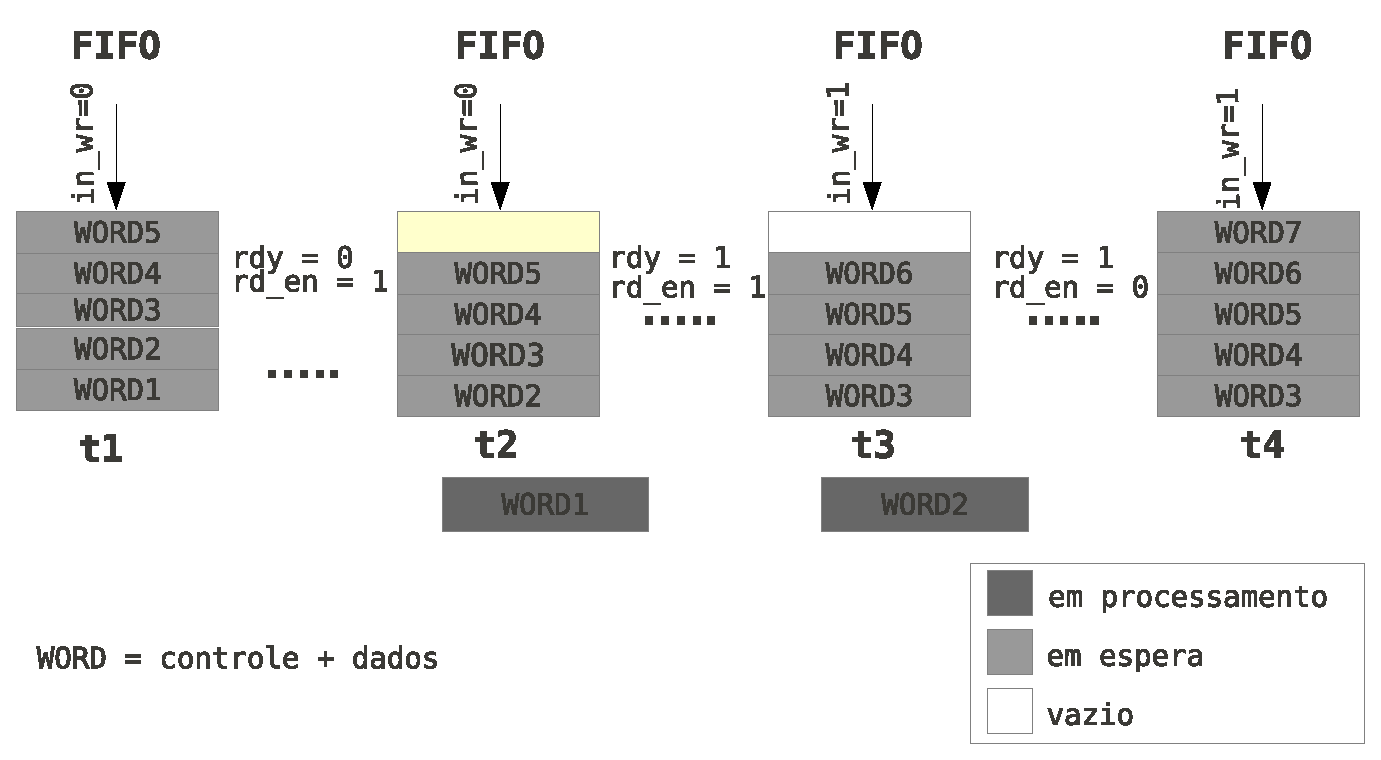
\includegraphics[scale=0.6,angle=0]{figures/modulos/fallthroughfifo.eps}
% \caption{Controle da fila de dados.}
% \label{fig:impl.fifo.msg}
% \end{figure}

\subsubsection{Máquina de estados}

Nosso \emph{firewall} implementa uma máquina de estados para verificar
se o pacote é IP e TCP.  Em caso positivo, a máquina de estados verifica
se a porta de destino deve ser filtrada e decide entre encaminhar ou
descartar o pacote.

Como todo o pacote é transmitido no barramento de encaminhamento com os
bits de controle zerados, nossa máquina de estado precisa manter
informação de qual palavra de 64~bits está sendo recebida.  Por exemplo,
como o cabeçalho IP e TCP somam pelo menos 40~bytes (56 bytes
contabilizando o cabeçalho Ethernet), o cabeçalho do pacote é recebido
ao longo de pelo menos cinco ciclos de relógio.  A
tabela~\ref{tab:impl.state.pktwords} mostra quais dados são transferidos
no barramento de encaminhamento a cada ciclo de relógio quando as linhas
de controle estão zeradas.

\begin{table}
\centering
\begin{tabular}{c|p{2.9cm}|p{2.9cm}|p{2.9cm}|p{2.9cm}|}
& \multicolumn{4}{c}{\ssf{in\_data}} \\
	Palavra & \multicolumn{1}{|c|}{\ssf{63:48}}     & \multicolumn{1}{|c|}{\ssf{47:32}}     & \multicolumn{1}{|c|}{\ssf{31:16}} & \multicolumn{1}{|c|}{\ssf{15:0}} \\ \hline
	1       & \multicolumn{3}{|l|}{Eth source addr} & Eth dest addr \\ \hline
	2       & \multicolumn{2}{|l|}{Eth dest addr}   & EtherType                             & IPver, HL, ToS \\ \hline
	3       & packet size                          & IP ID                                 & flags, frag                       & TTL, proto \\ \hline
	4       & checksum                             & \multicolumn{2}{|c|}{source IP}       & destination IP \\ \hline
	5       & destination IP                              & source port                          & destination port                         & seq. no. \\ \hline
	6       & seq. no.                             & \multicolumn{2}{|c|}{acknowledgement} & flags \\ \hline
	7       & adv. window                          & checksum                              & urgent ptr.                       & payload \\ \hline
	$\cdots$ & \multicolumn{4}{|l|}{payload} \\
\end{tabular}
\caption{Pacotes são encaminhados em palavras de 64 bits ao longo de
vários ciclos de relógio.  Na tabela um exemplo de pacote TCP.}
\label{tab:impl.state.pktwords}
\end{table}

\subsubsection*{Visão geral e atribuições padrão}

A figura~\ref{fig:impl.state.machine} mostra a máquina de estados do
nosso \emph{firewall}.  A ideia básica é receber o cabeçalho do pacote
para verificar se ele precisa ser descartado antes de transmiti-lo ao
próximo módulo.  Para receber e armazenar o cabeçalho do pacote
precisamos de uma fila de saída auxiliar, onde colocamos as palavras de
dados que já recebemos até decidir se devemos enviar o pacote para o
módulo seguinte ou descartá-lo.  A definição da fila de saída, mostrada
a seguir, é similar à definição da fila de entrada.

\begin{verilogcode}
   fallthrough_small_fifo #(
      ...
   ) output_fifo (
      .din           (out_fifo_din),   // Data in
      .wr_en         (out_fifo_wr),    // Write enable
      .rd_en         (out_fifo_rd_en), // Read the next word
      .dout          (out_fifo_dout),
      .full          (),
      .nearly_full   (out_fifo_nearly_full),
      .empty         (out_fifo_empty),
      .reset         (reset),
      .clk           (clk)
   );
\end{verilogcode}

A cada ciclo de relógio fazemos atribuições padrão que podem ser
sobrescritas dependendo do estado.  Em particular, deixamos a fila de
entrada travada, não escrevemos na fila de saída, e não repassamos dados
para o próximo módulo do \emph{pipeline}.  Também atribuímos os dados de
entrada da fila de saída aos dados retirados da fila de entrada.  Por
último, repassados ao próximo módulo no \emph{pipeline} os dados
retirados da fila de saída.

\begin{verilogcode}
    in_fifo_rd_en = 0;
    out_fifo_wr = 0;
    out_fifo_rd_en = 0;
    out_wr = 0;
    out_fifo_din = {in_fifo_ctrl, in_fifo_data};
    {out_ctrl, out_data} = out_fifo_dout;
\end{verilogcode}

\begin{figure}\centering
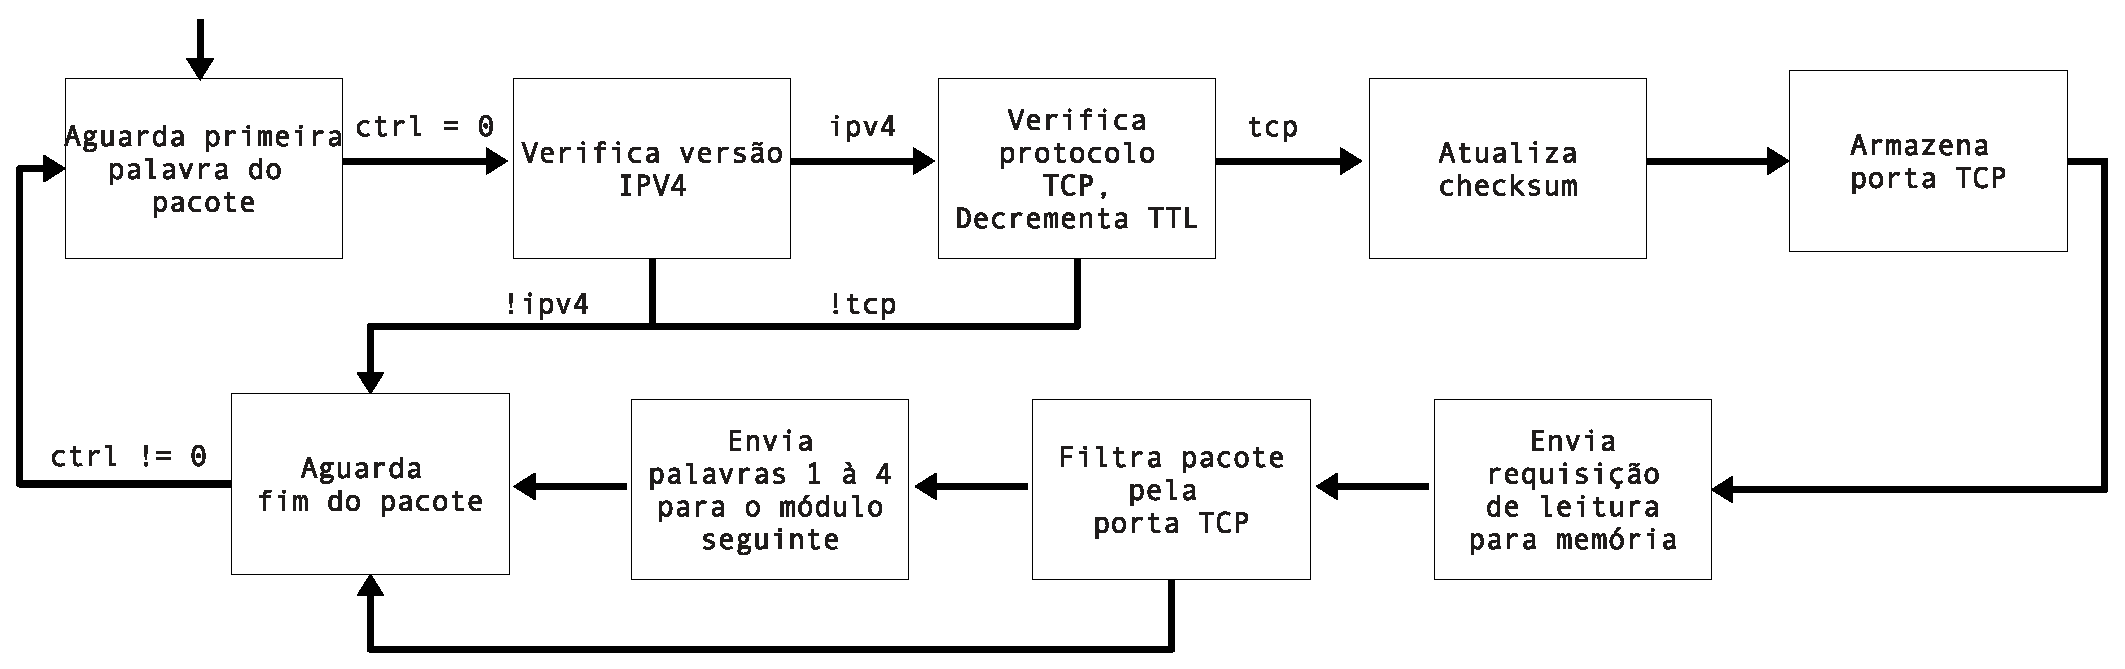
\includegraphics[scale=0.4]{figures/modulos/mestados.eps}
\caption{Máquina de estados do \emph{firewall}.}
\label{fig:impl.state.machine}
\end{figure}

Nossa máquina de estados atualiza todos os registradores a cada ciclo do
relógio.  Para cada registrador, temos um conjunto de linhas com o mesmo
nome e o sufixo \ssf{next}.  As linhas com sufixo \ssf{next} são
atribuídas aos respectivos registradores a cada ciclo do relógio.  Para
manter os valores nos registradores, inicializamos as linhas \ssf{next}
com o valor atual dos registradores e modificamos o valor das linhas
\ssf{next} em estados específicos quando necessário.

% \begin{minted}{verilog}
%       state_next = state;
%       save_1st_word_next = save_1st_word;
%       save_2nd_word_next = save_2nd_word;
%       save_3rd_word_next = save_3rd_word;
%       save_4th_word_next = save_4th_word;
%       dst_port_next = dst_port;
%       rd_0_req_next = 0;
%       num_TCP = num_TCP_next;
%       rd_0_addr_next = rd_0_addr;
%       drop_next = drop;
%       word_saved_next = word_saved;
% \end{minted}

\subsubsection*{Primeiro estado: esperando o início de pacotes}

O primeiro estado da nossa máquina de estados, \ssf{WAIT\_PACKET},
simplesmente espera o início do recebimento de um pacote, isto é, espera
as linhas de controle serem zeradas.  A implementação do primeiro
estado, mostrada abaixo, primeiro verifica se existe pacote a processar
e se o próximo módulo está pronto para receber pacotes verificando
\ssf{in\_fifo\_empty} e \ssf{out\_rdy}, respectivamente.  Se não há dado
a processar ou se o próximo módulo não está pronto para receber,
continuamos neste estado sem avançar as filas de entrada e saída (linha
12).  Se há dado a processar e o próximo módulo está pronto para
recebê-lo, nossa máquina de estados avança a fila ligando o sinal
\ssf{in\_fifo\_rd\_en} e grava os dados na fila de saída ligando
\ssf{out\_fifo\_wr}.  Se os bits de controle \ssf{in\_fifo\_ctrl} não
estiverem zerados, significa que ainda estamos recebendo metadados e o
início do pacote ainda não chegou.  Quando os bits de controle estiverem
zerados significa que acabamos de receber a primeira palavra de dados do
pacote (que contém o endereço MAC da origem,
tabela~\ref{tab:impl.state.pktwords}) e passamos para o segundo estado.

\begin{verilogcode}
  WAIT_PACKET: begin
     if (!in_fifo_empty && out_rdy) begin
        in_fifo_rd_en = 1;
        out_fifo_wr = 1;
        if(in_fifo_ctrl == 'h0) begin
           state_next = WORD2_CHECK_IPV4;
        end else begin
           state_next = WAIT_PACKET;
        end
     end
     else
        state_next = WAIT_PACKET;
  end
\end{verilogcode}


\subsubsection*{Segundo estado: verificação do protocolo de rede}

O segundo estado nosso \emph{firewall} processa a segunda palavra do
pacote e verifica se o pacote é um pacote IPv4.  Para isso verificamos
se o tipo do cabeçalho Ethernet (EtherType) é \ssf{0x0800}, que indica
um pacote IP, e se a versão do protocolo IP é \ssf{4}.\footnotemark{}
Em caso positivo, prosseguimos para o próximo estado para verificar se o
pacote é um pacote TCP.  Caso o pacote não seja um pacote IPv4 ele
deverá ser encaminhado pela rede sem ser filtrado.  Para encaminharmos o
pacote pulamos para o oitavo estado, \ssf{EMPTY\_OUT\_FIFO}, descrito
abaixo.

\footnotetext{Note que nosso \emph{firewall} não suporta VLANs (802.1Q).
Para tal seria necessário considerar o caso onde o EtherType é
\ssf{0x8100}.}

\begin{verilogcode}
  WORD2_CHECK_IPV4: begin
     if (!in_fifo_empty && out_rdy) begin
        if(in_fifo_data[31:16] != 16'h0800 ||
              in_fifo_data[15:12] != 4'h4) begin
           state_next = EMPTY_OUT_FIFO;
        end
        else begin
           in_fifo_rd_en = 1;
           out_fifo_wr = 1;
           state_next = WORD3_CHECK_TCP_TTL;
        end
     end
     else
        state_next = WORD2_CHECK_IPV4;
  end
\end{verilogcode}

\subsubsection*{Terceiro estado: verificação do protocolo de transporte}

No terceiro estado inspecionamos o cabeçalho IP para ver se o valor do
campo protocolo é \ssf{0x06}, que indica TCP.  Em caso negativo o pacote
é aceito: pulamos para o estado \ssf{EMPTY\_OUT\_FIFO} para enviarmos as
duas primeiras palavras mais metadados que foram armazenadas na fila de
saída (linha 9).  Note que, em caso negativo, a fila de entrada fica
bloqueada com a terceira palavra, que será transmitida após esvaziarmos
a fila de saída no estado \ssf{EMPTY\_OUT\_FIFO}.  Em caso positivo,
encaminhamos a terceira palavra para a fila de saída e passamos para o
próximo estado.

\begin{verilogcode}
  WORD3_CHECK_TCP_TTL: begin
     if (!in_fifo_empty && out_rdy) begin
        if(in_fifo_data[7:0] == 8'h06) begin
           in_fifo_rd_en = 1;
           out_fifo_wr = 1;
           state_next = WORD4_ADDR_CHKSUM;
        end
        else
           state_next = EMPTY_OUT_FIFO;
     end
     else
        state_next = WORD3_CHECK_TCP_TTL;
  end
\end{verilogcode}

\subsubsection*{Quarto estado: armazenamento dos endereços IP}

O quarto estado do \emph{firewall} armazena os dados da quarta palavra
do pacote temporariamente até verificarmos o número da porta de destino
no protocolo TCP no próximo estado.

\begin{verilogcode}
  WORD4_ADDR_CHKSUM: begin
     if (!in_fifo_empty && out_rdy) begin
        in_fifo_rd_en = 1;
        out_fifo_wr = 1;
        state_next = WORD5_TCP_PORT;
     end
     else
        state_next = WORD4_ADDR_CHKSUM;
  end
\end{verilogcode}

\subsubsection*{Quinto, sexto e sétimo estágios: verificando porta de
destino}

No quinto estado a fila de entrada contém a quinta palavra do pacote,
que possui o número da porta de destino do protocolo TCP.  Nós mantemos
as filas de entrada e saída travadas, armazenamos a porta de destino no
registrador \ssf{dst\_port} e avançamos para o próximo estágio.

\begin{verilogcode}
  WORD5_TCP_PORT: begin
     if (!in_fifo_empty && out_rdy) begin
        // in_fifo_rd_en and out_fifo_wr are zero by default
        dst_port_next = in_fifo_data[31:16];
        state_next = CHECK_RULES;
     end
     else
        state_next = WORD5_TCP_PORT;
  end
\end{verilogcode}

No sexto estágio mantemos as filas de entrada e saída travadas e
enviamos uma requisição de leitura da memória.  O endereço lido é
\ssf{SRAM\_PORTS\_ADDR}, que é definido igual a zero (primeira linha da
memória) e contém as portas de destino que estão bloqueadas.  Nós lemos
as portas bloqueadas da memória para ilustrar o acesso à memória SRAM e
porque as portas bloqueadas podem ser alteradas assincronamente pelo
usuário.  Na seção~\ref{sec:impl.mem} iremos detalhar o acesso à
memória.

\begin{verilogcode}
  CHECK_RULES: begin
     sram_rd_req_next = 1;
     sram_rd_addr_next = SRAM_PORTS_ADDR;
     state_next = CHECK_PORTS;
  end
\end{verilogcode}

Por último, o sétimo estágio espera a memória SRAM retornar os dados
verificando o valor de \ssf{rd\_vld}.  Esta espera é necessária pois a
SRAM demora alguns ciclos de relógio para retornar o dado requisitado.
Uma versão otimizada do nosso \emph{firewall} poderia realizar a
requisição de memória antes para evitar esta espera.  Se a porta de
destino for uma das portas bloqueadas, ligamos o registrador \ssf{drop}.
Independente da porta de destino passamos para o próximo estágio, onde a
fila de saída será esvaziada e os dados transmitidos para o próximo
módulo dependendo do valor do registrador \ssf{drop}.

\begin{verilogcode}
      CHECK_PORTS: begin
         if (rd_0_vld) begin
            if(sram_rd_data[15:0] == dst_port ||
                   sram_rd_data[31:16] == dst_port ||
                   sram_rd_data[47:32] == dst_port ||
                   sram_rd_data[63:48] == dst_port)
               drop_next = 1;
            else
               drop_next = 0;
            state_next = EMPTY_OUT_FIFO;
         end
         else
            state_next = CHECK_PORTS;
      end
\end{verilogcode}

\subsubsection*{Oitavo estágio: processando palavras armazenadas
temporariamente}

O oitavo estágio é responsável por processar os metadados e dados do
pacote armazenados temporariamente na fila de saída para o módulo
seguinte do \emph{pipeline}.  A cada ciclo de relógio processamos uma
palavra da fila de espera (linha 6).  Se o registrador \ssf{drop}
estiver desligado, enviamos uma palavra da fila de espera para o próximo
módulo (linha 7).  Se o registrador \ssf{drop} estiver ligado, retiramos
os dados da fila sem repassá-los ao módulo seguinte, efetivamente
descartando o pacote.  Quando a fila de espera estiver vazia pulamos
para o último estado onde enviamos o restante do pacote (a partir da
quinta palavra) para o próximo módulo diretamente da fila de entrada.

\begin{verilogcode}
      EMPTY_OUT_FIFO: begin
         if(!out_rdy)
            state_next = EMPTY_OUT_FIFO;
         else if(!out_fifo_empty) begin
            state_next = EMPTY_OUT_FIFO;
            out_fifo_rd_en = 1;
            out_wr = ~drop;
         end
         else
            state_next = PAYLOAD;
      end
\end{verilogcode}

\subsubsection*{Nono estágio: processando o conteúdo do pacote}

O nono e último estágio processa o resto do pacote a partir da fila de
entrada.  Os dados retirados da fila de entrada são repassados para o
próximo módulo dependendo do valor de \ssf{drop}.  Voltamos para o
primeiro estado quando detectamos o início do próximo pacote.
Detectamos o início do próximo pacote quando os bits de controle têm o
valor \ssf{IO\_QUEUE\_STAGE\_NUM}, do metadado adicionado pelas filas de
entrada quando o pacote é recebido na NetFPGA.  Note que assim que
detectamos o início do próximo pacote travamos a fila de entrada para
que a primeira palavra do pacote seja processada pelo primeiro estado do
\emph{firewall}.

\begin{verilogcode}
      PAYLOAD: begin
         if (!in_fifo_empty && out_rdy) begin
            {out_ctrl, out_data} = {in_fifo_ctrl, in_fifo_data};
            if(in_fifo_ctrl != `IO_QUEUE_STAGE_NUM)
                in_fifo_rd_en = 1;
                out_wr = ~drop;
                state_next = PAYLOAD;
            else begin
               in_fifo_rd_en = 0;
               out_wr = 0;
               drop_next = 0;            // reset drop register
               state_next = WAIT_PACKET;
            end
         end
         else
            state_next = PAYLOAD;
      end
\end{verilogcode}




\subsection{Modificação de pacotes em trânsito}
\label{sec:impl.mod}

Uma das funcionalidades da NetFPGA é a capacidade de modificar pacotes
em trânsito.  Iremos ilustrar essa funcionalidade decrementando o tempo
de vida (\emph{time to live}, TTL) do pacote.  Iremos também recalcular
o \emph{checksum} do pacote.  Para tanto vamos estender o código
apresentado na subseção anterior.

O tempo de vida do pacote é transmitido na terceira palavra
(figura~\ref{tab:impl.state.pktwords}).  Nosso \emph{firewall} processa
a terceira palavra do pacote no quarto estado (\ssf{WORD4\_ADDR\_TTL}).
Para decrementar o tempo de vida, iremos modificar o dado do pacote
antes de inseri-lo na fila de saída, como segue:

\begin{verilogcode}
      WORD3_CHECK_TCP_TTL: begin
         if (!in_fifo_empty && out_rdy) begin
            if(in_fifo_data[7:0] == 8'h06) begin
               in_fifo_rd_en = 1;
               out_fifo_wr = 1;
               out_fifo_din = {in_fifo_ctrl, in_fifo_data[63:16],
                               in_fifo_data[15:8] - 8'h1,
                               in_fifo_data[7:0]};
               state_next = WORD4_ADDR_CHKSUM;
            end
            else
               state_next = EMPTY_OUT_FIFO;
         end
         else
            state_next = WORD3_CHECK_TCP_TTL;
      end
\end{verilogcode}

De forma similar, precisamos atualizar o \emph{checksum} do pacote
devido ao decremento do tempo de vida.  Como o \emph{checksum} do
protocolo IP é simplesmente uma soma, podemos atualizá-lo simplesmente
somando o que foi subtraído devido ao decremento do tempo de
vida.\footnotemark{} No código abaixo, \ssf{chksum} possui 17~bits para
conseguirmos somar o \emph{carry out} em \ssf{\tt chksum\_cout}, que
possui 16~bits.

\footnotetext{O cálculo do \emph{checksum} do protocolo IP é detalhado
no RFC1071.  Ele depende do valor da soma das palavras de 2~bytes dos
campos do cabeçalho usando complemento de um.  Como o tempo de vida tem
apenas 1~byte e está alinhado com o byte mais significativo da palavra
de 2~bytes que o contém, nós incrementamos o byte mais significativo do
\emph{checksum}, somando \sssf{0x0100}, para compensar.}

\begin{verilogcode}
      assign chksum = {0, in_fifo_data[63:48]} + 16'h0100;
      assign chksum_cout = chksum[15:0] + {15'h0, chksum[16]};
        ...
      WORD4_ADDR_CHKSUM: begin
        if (!in_fifo_empty && out_rdy) begin
            in_fifo_rd_en = 1;
            out_fifo_wr = 1;
            in_out_fifo_dout = {in_fifo_ctrl, chksum_cout,
                        in_fifo_data[47:0]};
            state_next = WORD5_TCP_PORT;
        end
        else
            state_next = WORD4_ADDR_CHKSUM;
      end
\end{verilogcode}


\subsection{Acesso à memória SRAM}
\label{sec:impl.mem}

Nosso módulo utiliza a memória SRAM para armazenar as portas bloqueadas
e decidir quais pacotes filtrar.  No sexto estado do processamento de um
pacote emitimos uma requisição de leitura para o endereço
\ssf{SRAM\_PORTS\_ADDR}, que contem as portas TCP bloqueadas.  No sétimo
estado esperamos a leitura completar e então utilizamos o dado lido para
verificar se o pacote precisa ser descartado ou não.

Nosso \emph{firewall} emite operações de leitura da memória para o
módulo \ssf{sram\_arbiter}, que intermedia o acesso à memória SRAM.  As
linhas de comunicação do nosso \emph{firewall} com o \ssf{sram\_arbiter}
ilustram a interface de acesso à memória.

\begin{verilogcode}
      output reg                       sram_rd_req,
      output reg [SRAM_ADDR_WIDTH-1:0] sram_rd_addr,
      input [DATA_WIDTH-1:0]           sram_rd_data,
      input                            sram_rd_ack,
      input                            sram_rd_vld,
      output reg                       sram_wr_req,
      output reg [SRAM_ADDR_WIDTH-1:0] sram_wr_addr,
      output reg [DATA_WIDTH-1:0]      sram_wr_data,
      input                            sram_wr_ack,
\end{verilogcode}

O \ssf{sram\_arbiter} pode receber uma requisição de leitura ou escrita
por ciclo de relógio.  Requisições de leitura são indicadas ligando
\ssf{sram\_rd\_req} e informando o endereço a ser lido em
\ssf{sram\_rd\_addr}.  No próximo ciclo de relógio o \ssf{sram\_arbiter}
indica se a requisição foi recebida com sucesso ligando o sinal
\ssf{sram\_rd\_ack}.  Como leituras demoram alguns ciclos para serem
atendidas, o módulo que pediu a leitura deve esperar os dados serem
retornados e disponibilizados pelo \ssf{sram\_arbiter}.  O
\ssf{sram\_arbiter} informa que os dados estão disponíveis em
\ssf{sram\_rd\_data} ligando \ssf{sram\_rd\_vld}.

Requisições de escrita são indicadas ligando \ssf{sram\_wr\_req},
informando o endereço a ser escrito em \ssf{sram\_wr\_addr} e informando
o dado a ser escrito em \ssf{sram\_wr\_data}.  O \ssf{sram\_arbiter}
indica se a requisição foi recebida com sucesso ligando o sinal
\ssf{sram\_wr\_ack}.  Como o dado a ser escrito é armazenado pelo
\ssf{sram\_arbiter}, o módulo que fez a requisição de escrita não
precisa esperar mais nenhuma confirmação do \ssf{sram\_arbiter}.  Se
ambos os sinais \ssf{sram\_rd\_req} e \ssf{sram\_wr\_req} estiverem
ligados, nosso \ssf{sram\_arbiter} prioriza a requisição de escrita.  A
SRAM usada na NetFPGA garante que leituras realizadas após escritas
lerão o dado atualizado.

A interface que exportamos em nosso \ssf{sram\_arbiter} é simplificada.
Como descrito na seção~\ref{sec:arch.hw}, a NetFPGA possui dois bancos
de memórias SRAM, cada um com $2^{19}$ linhas de 36~bits.  Nosso
\ssf{sram\_arbiter} combina os dois bancos para apresentar uma abstração
de memória de $2^{19}$ linhas de 64~bits.  Usamos 8~bits de cada linha
como bits de paridade, calculados e verificados automaticamente pelo
\ssf{sram\_arbiter}.

\begin{verilogcode}
   // sram_arbiter.v
   generate
      genvar m;
      for(m = 0; m < 8; m = m+1) begin: calc_par_bits
      assign parbit[m] = wr_data[m*8] ^ wr_data[m*8+1] ^
            wr_data[m*8+2] ^ wr_data[m*8+3] ^ wr_data[m*8+4] ^
            wr_data[m*8+5] ^ wr_data[m*8+6] ^ wr_data[m*8+7];
      end // wr_data is 64 bits wide
   endgenerate 
   generate
      genvar l;
      for(l = 0; l < 8; l = l+1) begin: expand_wr_data
         assign wr_data_exp[(l+1)*9-1 : l*9] =
            {wr_data[(l+1)*8-1:l*8], parbit[l]};
         end // wr_data_exp is 72 bits wide (36*2)
   endgenerate
\end{verilogcode}

Para acessar as duas memórias simultaneamente duplicamos os sinais de
requisição de escrita ou leitura e os endereços para os dois bancos de
memória.  Para requisições de escrita escrevemos metade dos dados em
cada banco e para requisições de leitura concatenamos os dados dos dois
bancos.  Abaixo mostramos o código para realizar estas operações.  Este
código fica dentro do módulo \ssf{nf2\_core}.  O módulo \ssf{nf2\_core}
é o módulo raiz do \emph{software} da NetFPGA e comunica diretamente com
os pinos do FPGA.  O \ssf{nf2\_core} conecta os pinos do FPGA conectados
às memórias SRAM ao \ssf{sram\_arbiter} da seguinte forma.

\begin{verilogcode}
// nf2_core.v
// hardware pins       sram_arbiter
assign sram1_wr_data = wr_data_exp[`SRAM_DATA_WIDTH-1:0];
assign sram2_wr_data = wr_data_exp[2*`SRAM_DATA_WIDTH-1:`SRAM_DATA_WIDTH];
assign sram1_we      = sram_we; // 0 for write, 1 for read
assign sram2_we      = sram_we;
assign sram1_addr    = sram_addr;
assign sram2_addr    = sram_addr;
// sram_arbiter        hardware pins
assign sram_rd_data  = {sram2_rd_data, sram1_rd_data};
\end{verilogcode}

O \ssf{sram\_arbiter} pode ser modificado para permitir acesso mais
eficiente à memória caso a aplicação tenha um padrão específico de
acessos.  Por exemplo, é possível modificar as atribuições acima para
permitir ler endereços distintos em cada banco de SRAM.  A SRAM também
provê um mecanismo para permitir escritas parciais, escolhendo quais
bytes devem ser escritos em uma requisição de escrita.\footnotemark{}

\footnotetext{Não mostramos esta funcionalidade no texto.  Nossa
implementação não suporta escritas parciais.  Escritas parciais poderiam
ser controladas configurando o valor das linhas \sssf{sram\_bw} no
\sssf{sram\_arbiter}.}

Para exemplificar o controle de acesso à SRAM num nível mais baixo,
iremos explicar o tratamento de uma requisição de leitura (requisições
de escrita são mais simples).  Quando o \ssf{sram\_arbiter} recebe uma
requisição de leitura, ele desabilita escrita ligando o sinal
\ssf{sram\_we} (este sinal possui lógica negativa), repassa o endereço a
ser lido ao \emph{hardware} e confirma a requisição de leitura.

\begin{verilogcode}
   // sram_arbiter.v
   else if(sram_rd_req) begin
      hw_we <= 1'b1;                // read
      hw_addr <= sram_rd_addr;
      sram_rd_ack <= sram_rd_req;   // acknowledge read request
      sram_wr_ack <= 0;             // do not acknowledge write
      rd_vld_early3 <= sram_rd_req; // data back in three cycles
      ...
   end
\end{verilogcode}

Como o dado demora dois ciclos para ser retornado da SRAM após a
requisição, o \ssf{sram\_arbiter} possui um \emph{pipeline} interno para
esperar os dados serem retornados pela SRAM.  Após dois ciclos o
\ssf{sram\_arbiter} armazena o dado lido no registrador
\ssf{sram\_rd\_data} e encaminha este registrador para o \emph{firewall}
no terceiro ciclo de relógio após a requisição.

\begin{verilogcode}
   // sram_arbiter.v
   rd_vld_early2 <= rd_vld_early3; // waited 1
   rd_vld_early1 <= rd_vld_early2; // waited 2
   if(rd_vld_early1) begin // memory sending data this cycle, storing
      if(parity_check)
         sram_rd_data <= rd_data_exp_parsed; // no parity bits
      else
         sram_rd_data <= 64'hdeadfeeddeadfeed;
   end
   sram_rd_vld <= rd_vld_early1;   // data is here, set valid bit
\end{verilogcode}


\subsection{Registradores e interface PCI}
\label{sec:impl.regs}

Nosso projeto define quatro registradores de \emph{software}, um para
cada porta de destino que deve ser bloqueada.  Estes registradores de
\emph{software} podem ser configurados dinamicamente a partir do espaço
de usuário.  Nós definimos os registradores no arquivo XML de
configuração do nosso projeto como abaixo.

\begin{minted}{xml}
<!-- netfpga/projects/firewall/include/project.xml -->
<nf:name>firewall</nf:name>
   <nf:prefix>firewall</nf:prefix>
   <nf:location>udp</nf:location>
   <nf:description>Registers for minifirewall</nf:description>
   <nf:blocksize>128</nf:blocksize>
   <nf:registers>
      <nf:register>
         <nf:name>dport1</nf:name>
         <nf:description>Blocked port 1</nf:description>
         <nf:type>generic_software32</nf:type>
      </nf:register>
      ...
   </nf:registers>
\end{minted}

O programa \ssf{nf\_register\_gen} processa os arquivos XML de
configuração de todos os módulos de um projeto, gera um identificador
para cada módulo, calcula requisitos de armazenamento para os
registradores de cada módulo e gera endereços virtuais para cada
registrador.\footnotemark{}  O endereço virtual de um registrador é
composto do identificador do módulo onde foi declarado e de seu
deslocamento dentro do bloco de memória reservado aos registradores do
módulo.  Como nosso \emph{firewall} possui quatro registradores de 32
bits para armazenar as portas TCP que estão bloqueadas, definimos um
bloco de registradores de 128 bits (\ssf{blocksize} na configuração
acima).  O tamanho do bloco de registradores define a quantidade de bits
necessárias para a parte de deslocamento do endereço dos registradores.

\footnotetext{O arquivo XML com a configuração global do \emph{firewall}
está em \url{netfpfa/projects/firewall/include/project.xml}.  Arquivos
com a configuração dos módulos estão no mesmo diretório.}

O \ssf{nf\_register\_gen} gera cabeçalhos Verilog, C, Python e Perl
contendo constantes que permitem endereçar os registradores em cada uma
destas linguagens.  Os arquivos de cabeçalho são necessários para
compilação de programas de usuário e sintetização do projeto em
\emph{hardware}.  O \ssf{nf\_register\_gen} pode ser executado com o
comando seguinte (os cabeçalhos são criados dentro da pasta
\ssf{netfpga/projects/firewall/lib/}):

\begin{minted}{bash}
netfpga/bin/nf_register_gen.pl --project firewall
\end{minted}

% \begin{table}[h]
% \centering
% \begin{tabular}{|l|l|l|}
% \hline
% \textbf{Macro}       & \textbf{Endereço Verilog} & \textbf{Endereço C} \\ \hline
% FIREWALL\_DPORT1 & 5'h0                      & 0x2000000           \\ \hline
% FIREWALL\_DPORT2 & 5'h1                      & 0x2000004           \\ \hline
% FIREWALL\_DPORT3 & 5'h2                      & 0x2000008           \\ \hline
% FIREWALL\_DPORT4 & 5'h3                      & 0x200000c           \\ \hline
% \end{tabular}
% \label{tab:impl.firewall.regs}
% \caption{Endereços virtuais em arquivos de cabeçalho C e Verilog dos registradores do firewall.}
% \end{table}

Os endereços virtuais de registradores em programas do usuário possuem
28~bits e independem do tipo do registrador (contador, \emph{software},
ou \emph{hardware}).  Como a NetFPGA interage com sistemas operacionais
de 32~bits, registradores maiores que 32 bits são particionados em
múltiplas palavras de 32~bits segundo o esquema mostrado nas colunas
``64~bits'' e ``128~bits'' na tabela~\ref{table:impl.regs.width}.

\begin{table}[h]
\centering
\begin{tabular}{llllll}
\multicolumn{2}{c}{\textbf{32 bits}} & \multicolumn{2}{c}{\textbf{64 bits}} & \multicolumn{2}{c}{\textbf{128 bits}} \\ \hline
\textbf{Macro}     & \textbf{Endereço} & \textbf{Macro}         & \textbf{Endereço} & \textbf{Macro}            & \textbf{Endereço} \\ \hline
\ssf{EX\_REG} & 0x2000004         & \ssf{EX\_REG\_LO} & 0x2000004         & \ssf{EX\_REG\_1\_LO} & 0x2000004   \\
                   &                   & \ssf{EX\_REG\_HI} & 0x2000008         & \ssf{EX\_REG\_1\_HI} & 0x2000008   \\
                   &                   &                        &                   & \ssf{EX\_REG\_2\_LO} & 0x200000c   \\
                   &                   &                        &                   & \ssf{EX\_REG\_2\_HI} & 0x2000010   \\
\end{tabular}
\caption{Exemplo do esquema de geração de nomes para registradores maiores que 32 bits.}
\label{table:impl.regs.width}
\end{table}

Registradores de \emph{software} podem ser escritos lidos e escritos
utilizando as funções \ssf{readReg} e \ssf{writeReg} definidas na
biblioteca de funções da NetFPGA (em \ssf{netfpga/lib}).  Por exemplo,
no nosso programa de configuração dinâmica das portas bloqueadas,
\ssf{nffw}, temos:

\begin{minted}{c}
   // netfpga/projects/firewall/sw/nffw.c
   writeReg(&nf2, FIREWALL_DPORT0_REG, dropped[0]);
   ...
   readReg(&nf2, FIREWALL_DPORT0_REG, &check[0]);
\end{minted}

A memória SRAM também pode ser acessada pela interface de registradores.
A primeira palavra da memória SRAM é mapeada no endereço virtual
\ssf{SRAM\_BASE\_ADDR}, e outras palavras podem ser acessadas
indiretamente a partir de \ssf{SRAM\_BASE\_ADDR}.  O seguinte exemplo
zera as dez primeiras palavras da memória:

\begin{minted}{c}
   for(i = 0; i < 10; i++)
      unsigned offset = i*4; // 4 bytes per word
      writeReg(&nf2, SRAM_BASE_ADDR + offset, 0);
\end{minted}

Chamadas de função como \ssf{writeReg} enviam uma requisição de escrita
em registrador para a NetFPGA.  Essa requisição é recebida pelo
barramento PCI.  Para facilitar o processamento de requisições de
escrita e leitura dos registradores, podemos usar o módulo
\ssf{generic\_regs}.  O módulo \ssf{generic\_regs} é padrão no pacote de
\emph{software} da NetFPGA e é instanciado dentro dos módulos que
compõem o \emph{pipeline} de processamento.

Quando instanciamos o \ssf{generic\_regs}, definimos o número de
registradores e as linhas conectadas a cada registrador.  Definimos
também em qual módulo ele está sendo instanciado (parâmetro \ssf{TAG}).
Esta informação permite à instância do \ssf{generic\_regs} identificar
os endereços dos registradores do módulo e quais requisições de escrita
e leitura em registradores deve tratar.

\begin{verilogcode}
   generic_regs
   #(
      .TAG               (`FIREWALL_BLOCK_ADDR), // module ID
      .NUM_SOFTWARE_REGS (4),                    // number of sw regs
      ...
   ) module_regs (
      .reg_req_in       (reg_req_in),      // register bus input lines
      .reg_ack_in       (reg_ack_in),
      .reg_rd_wr_L_in   (reg_rd_wr_L_in),
      .reg_addr_in      (reg_addr_in),
      .reg_data_in      (reg_data_in),
      .reg_src_in       (reg_src_in),
      .reg_req_out      (reg_req_out),     // register bus output lines
      .reg_ack_out      (reg_ack_out),
      .reg_rd_wr_L_out  (reg_rd_wr_L_out),
      .reg_addr_out     (reg_addr_out),
      .reg_data_out     (reg_data_out),
      .reg_src_out      (reg_src_out),
      .counter_updates  (),                // register definitions
      .counter_decrement(),
      .software_regs    ({dport1, dport2, dport3, dport4}),
      .hardware_regs    (),
      ...
    );
\end{verilogcode}

As requisições de leitura e escrita em registradores recebidas pelo
barramento PCI são inseridas no barramento de registradores.  O
barramento de registradores é paralelo ao barramento de encaminhamento.
Como no barramento de encaminhamento, cada instância do módulo
\ssf{generic\_regs} tem sinais de entrada (sufixo \ssf{\_in}), para
receber requisições do módulo anterior, e de saída (sufixo \ssf{\_out}),
para repassar as requisições ao próximo módulo.  Ilustramos o barramento
de registradores na figura~\ref{fig:impl.regs.bus}.  A linha \ssf{req}
indica se as outras linhas carregam uma requisição válida.  As linhas
\ssf{addr} especificam o endereço virtual do registrador.  A linha
\ssf{rd\_wr\_L} indica se a requisição é de leitura ou escrita (com
lógica negativa, leitura quando ligado e escrita quando desligado) e as
linhas \ssf{data} contém o dado a ser escrito ou o dado lido.  A linha
\ssf{ack} indica se a requisição já foi tratada e as linhas \ssf{src}
indicam qual módulo tratou a requisição.

\begin{figure}
\centering
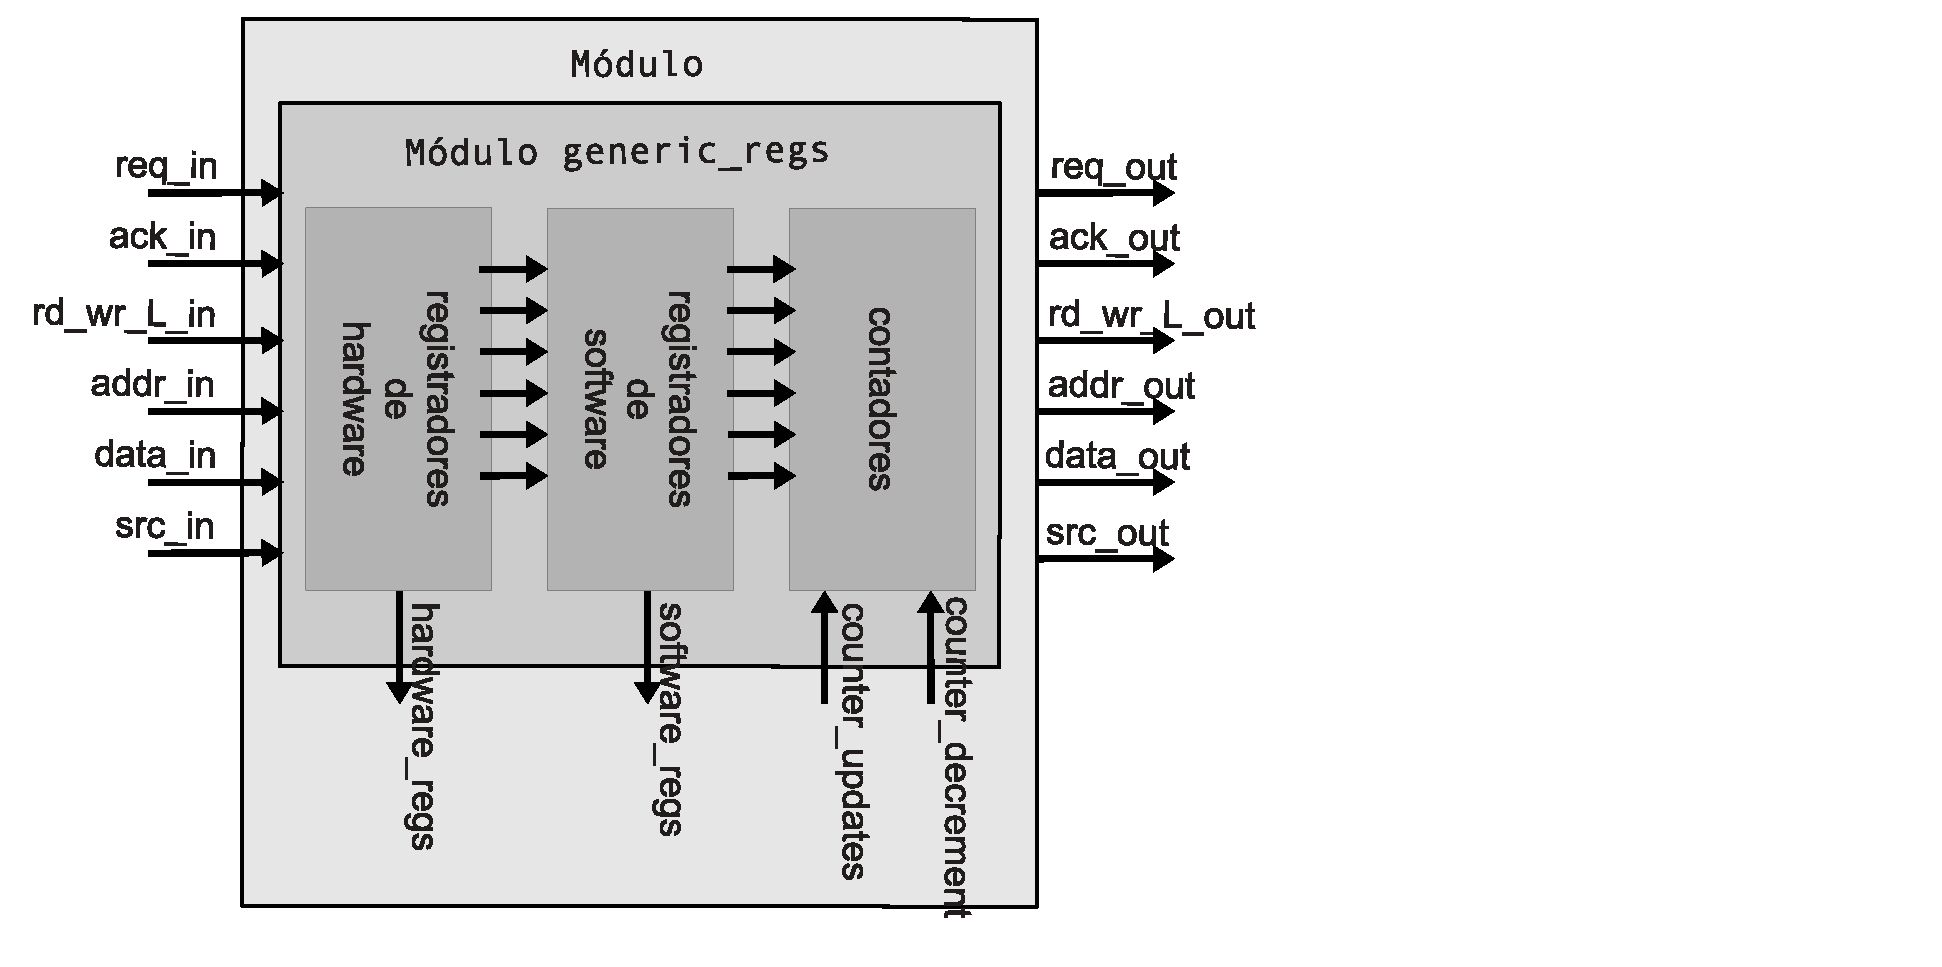
\includegraphics[scale=0.6,angle=0]{figures/modulos/genregister.eps}
\caption{Módulo \ssf{generic\_regs} e barramento de registradores.}
\label{fig:impl.regs.bus}
\end{figure}

O \ssf{nf\_register\_gen} gera blocos para armazenamento de
registradores automaticamente.  Para projetos com requisitos
específicos, é possível controlar o endereço base dos registradores de
cada módulo no arquivo XML de configuração do projeto.  Por exemplo,
para posicionar os registradores do nosso \emph{firewall} no endereço
\ssf{0x02000400} basta utilizar a configuração a seguir.

\begin{minted}{xml}
<!-- netfpga/projects/firewall/include/project.xml -->
<nf:memalloc layout="reference">
    <nf:group name="udp">
        <nf:instance name="firewall" base="0x02000400"/>
        ...
    </nf:group>
    ...
</nf:memalloc>
\end{minted}

Nosso \emph{firewall} lê as portas que devem ser filtradas da memória
SRAM (sexto estágio).  Esta decisão de projeto é didática, para
exemplificar a utilização da memória SRAM.  Num projeto real, as portas
poderiam ser lidas diretamente dos registradores \ssf{dport0},
\ssf{dport1}, \ssf{dport2}, \ssf{dport3}.  Para que possa ler as portas
TCP bloqueadas da memória SRAM, nosso \emph{firewall} precisa também
gravar esta informação na memória.  Isto é realizado gravando os
registradores na memória usando o módulo \ssf{sram\_arbiter}.  Para
detectar se as portas bloqueadas foram modificadas, verificamos se o uma
requisição de registrador foi atendida (\ssf{reg\_ack\_out}) e se o
endereço da requisição pertence ao nosso módulo (\ssf{tag\_hit} e
\ssf{addr\_good}).  Para verificar se o endereço da requisição pertence
ao nosso módulo, utilizamos as constantes geradas pelo
\ssf{nf\_register\_gen}.

\begin{verilogcode}
   always @(*) begin
      wr_data_next <= {dport3[15:0], dport2[15:0],
                       dport1[15:0], dport0[15:0]};
      wr_addr_next <= SRAM_PORTS_ADDR;
      if(tag_hit && addr_good && reg_ack_out)
         wr_req_next <= 1;
      else
         wr_req_next <= 0;
   end
   assign addr_block = reg_addr_out[`UDP_REG_ADDR_WIDTH-1:
                                    `FIREWALL_REG_ADDR_WIDTH];
   assign tag_hit = `FIREWALL_BLOCK_ADDR == addr_block;
   assign addr_good = reg_addr_out[`FIREWALL_REG_ADDR_WIDTH-1:0] >= 
    `FIREWALL_DPORT0 && reg_addr_out[`FIREWALL_REG_ADDR_WIDTH] <= 
    `FIREWALL_DPORT3;
\end{verilogcode}

As linhas \ssf{addr\_block} são construídas a partir do endereço da
requisição e contém o identificador do bloco de registradores (linha
10).  O identificador do bloco de registradores pode ser utilizado para
verificar se o registrador pertence ao nosso módulo (linha 12).  Por
último, a linha \ssf{addr\_good} indica se o registrador escrito é um
dos registradores que armazena as portas TCP bloqueadas (linha 13).


\subsection{Sistema de testes}
\label{sec:impl.test}

O \emph{software} da NetFPGA tem um \emph{framework} que projetos podem
utilizar para facilitar e automatizar o desenvolvimento e execução de
testes.

O programa \ssf{nf\_test.py} executa testes armazenados dentro do
subdiretório \ssf{test} no diretório do projeto apontado pela variável
de ambiente \ssf{NF\_DESIGN\_DIR}. O nome de cada teste deve seguir um
formato específico, indicando se é um teste de simulação (\ssf{sim}), um
teste do \emph{hardware} sintetizado (\ssf{hw}) ou ambos (\ssf{both}); o
componente sendo testado (\ssf{major}); e o teste específico
(\ssf{minor}).  Por exemplo, o comando abaixo irá executar o teste em
\ssf{projects/firewall/test/sim\_firewall\_tcp}.

\begin{minted}{bash}
# inside the NetFPGA root directory
export NF_DESIGN_DIR=$(pwd)/projects/firewall
bin/nf_test.py --isim --major firewall --minor tcp sim
\end{minted}

O \ssf{nf\_test.py} chama o \emph{script} \ssf{run.py} dentro do
diretório do teste.  Os \emph{scripts} \ssf{run.py} podem utilizar
funções da biblioteca de testes da NetFPGA.\footnote{As bibliotecas do
\emph{framework} de testes ficam no diretório \sssf{lib/python/NFTest}.
As funções relativas a manipulação de pacotes estão em
\sssf{PacketLib.py} e as funções relativas à comunicação via interface
PCI estão em \sssf{NFTestLib.py}.} A biblioteca possui funções que
permitem construir pacotes de rede usando a biblioteca
Scapy\footnote{Scapy, disponível em
\sssf{www.secdev.org/projects/scapy/}.} disponível no Python.  A
biblioteca injeta os pacotes gerados interfaceando com o simulador ou
com o \emph{hardware} dependendo do tipo de teste sendo realizado.  A
biblioteca também permite verificar se pacotes foram transmitidos ou
não.  No teste \ssf{sim\_firewall\_tcp} criamos pacotes TCP com
diferentes portas de destino e depois verificamos se os pacotes cujas
portas não estão bloqueadas foram encaminhados.  Caso pacotes sejam
erroneamente encaminhados ou descartados, o teste resultará em erro.

\begin{minted}{python}
   # projects/firewall/test/sim_firewall_tcp/run.py
   eth_hdr = scapy.Ether(dst=DA, src=SA)
   ip_hdr = scapy.IP(dst=DST, src=SRC)
   tcp_hdr = scapy.TCP(dport=random.choice(POSSIBLE_PORTS), sport=SPORT)
   ...
   pkt = eth_hdr/ip_hdr/tcp_hdr/payload
   nftest_send_phy('nf2c0', pkt)
   if(pkt.dport not in BLOCKED_PORTS):
      ...
      nftest_expect_dma('nf2c0', pkt)
\end{minted}

A biblioteca também possui funções que permitem escrever e ler valores
de registradores e da memória SRAM.  Para tornar o teste
\ssf{sim\_firewall\_tcp} interessante, utilizamos as funções da
biblioteca para configurar as portas que devem ser filtradas, bem como
verificar se a configuração foi escrita no registrador.  Note que o
módulo Python \ssf{reg\_defines} é gerado pelo \ssf{nf\_register\_gen}.

\begin{minted}{python}
# projects/firewall/test/sim_firewall_tcp/run.py
nftest_regwrite(reg_defines.FIREWALL_DPORT0_REG(),
                BLOCKED_PORTS[0])
nftest_regread_expect(reg_defines.FIREWALL_DPORT0_REG(),
                      BLOCKED_PORTS[0])
\end{minted}

Podemos também verificar se as portas foram escritas na primeira linha
de memória de onde nossa máquina de estados lê as portas que devem ser
bloqueadas.  Adicionamos um pequeno atraso no \emph{script} de teste
para dar tempo para os dados serem gravados na memória.  A manipulação
dos bits é necessária devido ao formato no qual as portas são gravadas
na memória SRAM.

\begin{minted}{python}
simReg.regDelay(1000)
nftest_regread_expect(reg_defines.SRAM_BASE_ADDR(),
                      BLOCKED_PORTS[2]<<16 | BLOCKED_PORTS[3])
\end{minted}

A saída do \ssf{nf\_test.py} contém o tempo de simulação e as mensagens
escritas.  Estas mensagens podem ser geradas de dentro do código Verilog
usando as diretivas \ssf{\$display}.  As funções disponibilizadas pelo
sistema de testes em Python geram mensagens indicando qual operação será
realizada e o seu resultado. Por exemplo, as asserções de leitura sobre
endereços definidos nos arquivos de cabeçalho normalmente produzem a
mensagem \emph{``Good: PCI read of addr X returned data Y as expected''}
quando o resultado está correto. O final da saída indica se todas as
verificações do teste passaram através da mensagem \emph{``Test X
passed!''} e vice-versa.

\begin{comment}
Os tempos de simulação estão indicados no começo da linha, seguido pelo dado que desejamos escrever e o endereços de destino nas operações de escrita, e o tempo, seguidos de endereço e dados nas operações de leitura. As quatro primeiras operações escrevem as portas que devem ser filtradas nos registradores correspondentes. \footnote{Os endereços em hexadecimal podem ser verificados no arquivo {\tt lib/Python/reg\_defines\_firewall.py}} As quatro primeiras operações de leitura verificam se os registradores receberam os dados, enquanto as duas últimas leituras conferem se a primeira linha da memória SRAM possui as portas que devem ser filtradas. No teste realizado acima preenchemos o vetor {\tt BLOCKED\_PORTS} com as portas 667, 22, 80 e 1210. É possível verificar que realmente são essas portas estão gravadas através do {\tt Python}:

\begin{minted}{python}
$ python
>>> 0x16029b&0xffff
667
>>> 0x16029b>>16&0xffff
22
>>> 0x4ba0050&0xffff
80
>>> 0x4ba0050>>16&0xffff
1210

\end{minted}

Podemos verifica o resultado das asserções (leitura dos registradores) através da busca do padrão textual {\tt Good}:

\begin{minted}{python}
 7455.00ns testbench.host32: Good: PCI read of addr 0x02000100 
                                    returned data 0x000004ba as expected.
23205.00ns testbench.host32: Good: PCI read of addr 0x02000104 
                                    returned data 0x00000050 as expected.
24015.00ns testbench.host32: Good: PCI read of addr 0x02000108 
                                    returned data 0x00000016 as expected.
24825.00ns testbench.host32: Good: PCI read of addr 0x0200010c 
                                    returned data 0x0000029b as expected.
26655.00ns testbench.host32: Good: PCI read of addr 0x01000000 
                                    returned data 0x0016029b as expected.
27465.00ns testbench.host32: Good: PCI read of addr 0x01000004 
                                    returned data 0x04ba0050 as expected.
29325.00ns testbench.host32: Good: PCI read of addr 0x00600008 
                                    returned data 0x00000008 as expected.
\end{minted}
\end{comment}


